%%%%%%%%%%%%%%%%%%%%%%% file typeinst.tex %%%%%%%%%%%%%%%%%%%%%%%%%
%
% This is the LaTeX source for the instructions to authors using
% the LaTeX document class 'llncs.cls' for contributions to
% the Lecture Notes in Computer Sciences series.
% http://www.springer.com/lncs       Springer Heidelberg 2006/05/04
%
% It may be used as a template for your own input - copy it
% to a new file with a new name and use it as the basis
% for your article.
%
% NB: the document class 'llncs' has its own and detailed documentation, see
% ftp://ftp.springer.de/data/pubftp/pub/tex/latex/llncs/latex2e/llncsdoc.pdf
%
%%%%%%%%%%%%%%%%%%%%%%%%%%%%%%%%%%%%%%%%%%%%%%%%%%%%%%%%%%%%%%%%%%%

\documentclass[runningheads,a4paper,10pt]{llncs}

\usepackage[utf8]{inputenc}
\usepackage[left=3cm,right=3cm,top=3cm,bottom=3cm]{geometry}

\usepackage{natbib}
\bibliographystyle{apalike-fr}

\usepackage{amssymb}
\setcounter{tocdepth}{3}
\usepackage{graphicx}

\usepackage{amsmath}

\usepackage[french]{babel} % Pour adopter les règles de typographie française
\usepackage[T1]{fontenc} % Pour que les lettres accentuées soient reconnues

\usepackage{url}
\urldef{\mailsa}\path|{alfred.hofmann, ursula.barth, ingrid.haas, frank.holzwarth,|
\urldef{\mailsb}\path|anna.kramer, leonie.kunz, christine.reiss, nicole.sator,|
\urldef{\mailsc}\path|erika.siebert-cole, peter.strasser, lncs}@springer.com|    
\newcommand{\keywords}[1]{\par\addvspace\baselineskip
\noindent\keywordname\enspace\ignorespaces#1}

\begin{document}

\mainmatter 

\title{Mini Mémoire \\ Le Model-Checking de CTL}

\titlerunning{Le Model-Checking de CTL}

\author{BUI QUANG PHUONG Linh -- 000427796 \\ Promoteur : GEERAERTS Gilles}

\institute{Université Libre de Bruxelles}

\authorrunning{BUI QUANG PHUONG Linh}

\toctitle{Abstract}
\tocauthor{{}}

\maketitle


\begin{abstract}
La vérification de modèles, plus communément appelée via son appellation anglaise \textit{Model-Checking}, est un système de vérification automatique qu'un système informatique ou électronique satisfasse une certaine propriété. Celle-ci est généralement utilisé afin de prouver la bonne fonctionnalité du système ou dans le cas contraire, de détecter des bugs ou des dysfonctionnements. Plusieurs types d'algorithmes et de logiques permettent d'effectuer un Model-Checking. Nous allons principalement nous intéresser au Model-Checking de CTL mis en place durant les années 80. 
\end{abstract}

\medskip

\begingroup
\let\clearpage\relax
\tableofcontents
\endgroup

\medskip
\medskip

\newpage 

\section{Introduction}

\subsection{Contexte et point de vue global}
\noindent
Les dernières décennies entrainant l'évolution exponentielle de la technologie et de l'informatique, la société actuelle fait régulièrement usage de systèmes automatisés afin d'assurer le bon fonctionnement et la fiabilité des programmes, machines et autres divers systèmes informatiques. Afin de vérifier ces systèmes, l'utilisation d'une technique algorithmique appelée \textit{Model-Checking} va être mise en place.  

\noindent
Le principe de base du model-checking est la vérification qu'un certain système satisfasse une certaine propriété. Le système sera représenté par un modèle \textit{M} tandis que la propriété fera office d'une formule $\Phi$. Dans un premier temps, la modélisation du comportement dynamique du système est nécessaire avant d'être suivie par la vérification de la formule de la propriété grâce à l'algorithme de model-checking qui déterminera si le modèle satisfait bien la formule.  

$$\boxed{\textit{M} \vDash \Phi}$$

\noindent
Lorsque le système ne satisfait pas la propriété évaluée, le model-checking a donc repéré un bug ou un dysfonctionnement. Chaque année, le coût des bugs s'élève à environ 59 milliards de dollars\footnote{Source: https://raygun.com/blog/cost-of-software-errors/} rien qu'aux Etats-Unis. La création et la mise en place de technique de vérification est donc impérative pour réduire le taux de bugs afin de minimiser ces coûts.  \\

\noindent
Illustrons cela par un exemple plus concret : un distributeur de boissons. Dans ce cas, il est indispensable que le montant demandé pour une certaine boisson soit mis dans la machine afin que le client puisse récupérer la boisson. La vérification de ce prérequis va être effectué à l'aide d'un système de model-checking. 
Un autre exemple illustrant l'importance du model-checking est la fermeture des barrières sur une voie ferrée lors du passage d'un train. 
Celle-ci doit être réalisée automatiquement lorsqu'un train est sur le point de traverser une voie ferrée. Dans ce cas, une petite erreur de timing peut avoir une très grande ampleur concernant la sécurité des passants. Il est donc impératif de vérifier la bonne fonctionnalité du système gérant la fermeture des barrières grâce au model-checking. 

\noindent 

\subsection{Les phases du model-checking}

Le processus de base d'un model-checking est divisé en 3 phases : 

\begin{enumerate}
 \item  \textbf{La phase de modélisation} : permet de représenter le comportement du système. Dans le cas du model-checking, cette phase de modélisation est réalisée à l'aide d'automates d'états finis et de logique temporelle. Celle-ci permet une formalisation du système ainsi que de la propriété à vérifier. De plus, cette modélisation permet de réaliser les premières vérifications grâce à différentes simulations réalisées sur le modèle. Cette phase de modélisation est l'objet de la section 2 \textit{"Point de vue algorithmique"}. 
 \item  \textbf{La phase d'exécution} : exécution du model-checker vérifiant la validité de la propriété à satisfaire. 
 \item  \textbf{La phase d'analyse} : lorsque les résultats sont obtenus après exécution, différents cas potentiels existent : 
 \begin{itemize}
 \item Si la propriété est \textbf{satisfaite} : vérification de la propriété suivante (si il y en a). 
 \item Si la propriété n'est \textbf{pas satisfaite} : soit un contre-exemple est produit qui décrit un scénario possible d’erreur (violation de la propriété), soit il y a correction du modèle et réexécution du model-checker, soit il y a réexécution de toute la procédure. 
 \item \textbf{Manque de mémoire} (cfr. \textit{State explosion problem}\footnote{Section 1.3 - 1er désavantage}): tentative de réduction du modèle notamment grâce aux diagrammes de décision binaire ou une réduction partielle de la commande et réexécution le model-checker. 
 \end{itemize}
 \end{enumerate} 
 
 \newpage
 
 \begin{figure}
  \centering
  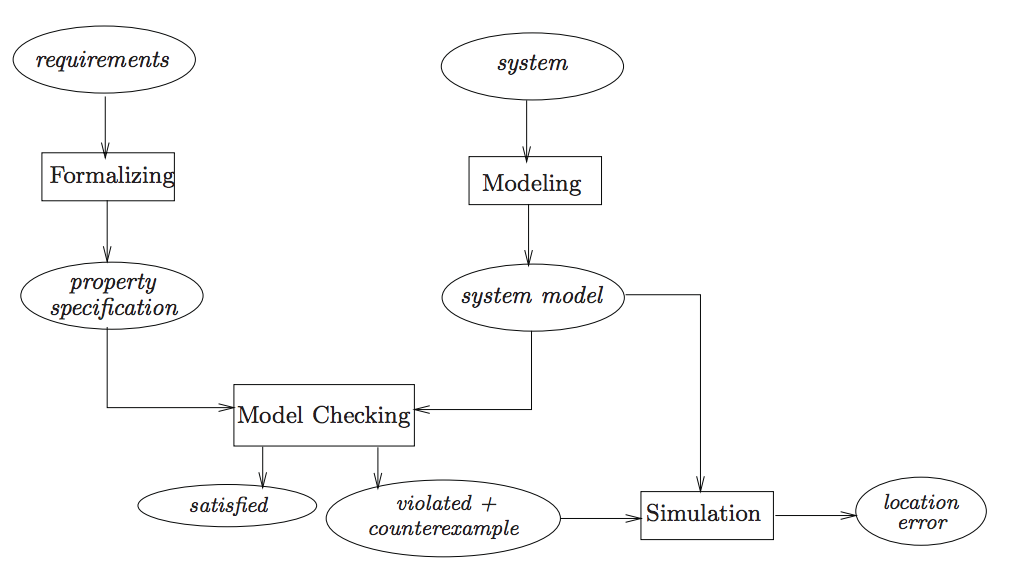
\includegraphics[scale=0.7]{schematic-view.png}
   \caption[Caption for LOF]{Vue schématique de l'approche du model-checking\protect\footnotemark}
\end{figure}

\footnotetext{Source: Christel Baier and Joost-Pieter Katoen, Principles of Model Checking, p.8 figure 1.4}

\subsection{Avantages \& désavantages}

\subsubsection{Avantages du model-checking}

Un model-checking possède plusieurs avantages par rapport à l'utilisation d'éventuelles autres techniques de vérifications et de détection d'erreur. Voici une liste non exhaustive de ces avantages : 

\begin{itemize}
\item Il s'agit d'une approche générale de vérification applicable dans tous les domaines tels que les systèmes embarqués ou ingénierie logicielle. 
\item La phase de vérification est automatique. Suivant la phase de modélisation, la seule action nécessaire de l'utilisateur afin de faire fonctionner le model-checking est de l'activer. Le programme s'occupe du reste. Niveau performance, cet automatisme permet un gain de temps conséquent. 
\item Contrairement aux simples tests, le model-checking va également prouver la bonne fonctionnalité du système et dans le cas contraire, nous renvoyer un contre-exemple d'une exécution du système qui falsifie la propriété et ainsi, détecter le(s) bug(s). Le taux d'erreurs non repérés est donc moindre par rapport aux tests simples. 
\item Le model-checking agit sur tout le système et non qu'une seule partie, il s'agit donc d'une méthode exhaustive. Néanmoins, si l'utilisateur le souhaite, il est tout de même possible d'utiliser le model-checking pour une vérification partielle et ainsi l'appliquer à des parties de système. 
\item Utilisation de la logique temporelle (\textit{cfr. section 3.1 "Logique temporelle"}) qui permet d'exprimer facilement les diverses propriétés. 
\end{itemize}

\subsubsection{Désavantages du model-checking}

Néanmoins, le model-checking est une solution discutable sur certains points : 

\begin{itemize}
\item Le model-checking grandit exponentiellement au nombre de processus actifs (appelés états, correspondant à la taille du système). Pour $N$ variables avec un domaine de $k$ valeurs possibles, le nombre d'états grandit de $k^{N}$. Par exemple, pour 20 variables booléennes, il y aurait déjà $2^{20}$ soit 1048576 états. Le modèle devient donc très vite surchargé et surpasse la capacité de la mémoire. Ce problème est appelé \textit{State explosion problem}. Par conséquent, le model-checking ne pourrait donc pas croître. Cependant, plusieurs recherches ont été établies dans le but d'établir une solution à ce problème tels que les \textit{diagrammes de décisions binaires} permettant de représenter plusieurs états en un diagramme. 
\item Le model-checking s'applique généralement sur des systèmes finis et n'est pas adapté aux systèmes non-finis de part sa modélisation grâce à des automates d'états finis. Hors, la possibilité de tomber sur un système non-fini (ayant donc une infinité de valeurs possibles pour les variables) n'est pas écartée. % EXPLIQUER PLUS
\item Comme son nom l'indique, le model-checking exécute une vérification du modèle du système et non du système en lui-même. Les résultats obtenus pour le modèle correspondent en grande partie au système réel, néanmoins, il est nécessaire d'utiliser des techniques supplémentaires comme des tests pour trouver les éléments qui pourraient différer entre le modèle et le système réel, que ce soit au niveau du hardware tel que des défauts de fabrication ou bien au niveau software tel que des erreurs de codage. 
\item Conséquence du dernier point : le résultat n'est donc pas garanti à 100\% et pourrait donc contenir des erreurs. 
\end{itemize}

\section{Point de vue algorithmique}

\subsection{Graphes et principes d'états}
Présentation du principe de systèmes d'états finis et de graphes en quelques mots + Schéma 

\subsection{Structure de Kripke}
Présentation de la structure de Kripke, définitions des différentes notions. 

\subsubsection{Application - exemple de modélisation à l'aide de la structure de Kripke}
Exemple d'une structure de Kripke + Schéma. Explication de l'exemple. 

\subsection{Arbre d'exécution d'une structure de Kripke}

\subsubsection{Pourquoi utiliser un arbre ?}
Expliquer pourquoi on passe d'un graphe à un arbre? Quel est en l'utilité? 

\subsubsection{Application - du graphe à l'arbre}
Traduction de l'exemple de Kripke donné ci-dessus en arbre. 

\section{Le model-checking de CTL: généralités et logiques}

\subsection{Introduction à la logique temporelle}
Première approche de la notion de logique temporelle, des différentes sortes de logiques temporelles existantes (linéaire ou arborescente), des propositions de logiques temporelles, des formules associés, ... 

\subsubsection{LTL}
Aperçu et premier approche de la logique temporelle linéaire LTL 

\subsubsection{CTL}
Aperçu et premier approche de la logique temporelle linéaire CTL 

\subsection{Avantages d'une structure d'arbre}
Présentation des différents avantages de CTL

\subsubsection{Brève comparaison avec LTL}
Comparaison (avantages+désavantages) par rapport à LTL 

\subsubsection{Exemple d'arbre CTL}
Exemple d'un arbre CTL + explications

\subsection{Syntaxe}
Présentation détaillée de la syntaxe utilisée par CTL ainsi que ses différentes propriétés 

\subsection{Sémantique}
Présentation de la sémantique de CTL - des relations de satisfactions, des interprétations des différentes formules, etc.. 

\section{Le model-checking CTL: algorithme et implémentation}
\subsection{Pseudo-code de l'algorithme}
Pseudo-code (ou code personnel) simple d'un algorithme de Model Checking CTL. 

\subsection{Analyse du code}
Analyse détaillée du code de l'algorithme et exemple d'application 

\subsection{Complexité}
Complexité du code donné ainsi que d'un model checking de CTL en général \\ 

\textbf{FIN DU DOC: Sources, bibliographie} 

\bibliography{references}
\nocite{*} 

\end{document}
